%==============================================================================
% Chapter 03: Exceptional Lie Groups
% Source: Maximal_Extraction_SET1_SET2.md (lines 6700-7200, 18400-18900)
%         E8_Research_Survey_2010-2025.md (complete, 1730 lines)
% Date: 2025-10-21
% Status: Complete (transformed to whitepaper narrative style)
% Transformed: Matching Ch01 template (motivation-first, physical intuition)
%==============================================================================

\chapter{Exceptional Lie Groups: The Hidden Symmetries of Nature}
\label{ch:exceptional-lie-groups}
\index{exceptional Lie groups}
\index{Lie groups!exceptional}

%------------------------------------------------------------------------------
% OPENING NARRATIVE: The Quantum Magnet Discovery
%------------------------------------------------------------------------------

\section*{The Standard Model's Missing Link: Why Particle Physics Needs Exceptional Symmetries}

The Standard Model of particle physics is spectacularly successful. It predicted the Higgs boson (discovered 2012), the W and Z bosons (1983), the top quark (1995), and countless other phenomena with stunning precision. Yet it is incomplete. The theory has 19 free parameters that must be measured experimentally rather than predicted from first principles. Why these specific particle masses? Why three generations of fermions? Why this particular gauge group structure $\text{SU}(3)_C \times \text{SU}(2)_L \times \text{U}(1)_Y$?

Grand Unified Theories (GUTs)\index{Grand Unified Theory|see{GUT}}\index{GUT}\index{unification!gauge forces} attempt to answer these questions by embedding the Standard Model gauge group into a larger, simpler structure. The simplest candidate is $\text{SU}(5)$, proposed by Georgi and Glashow in 1974. At high energies (the GUT scale, approximately $10^{16}$ GeV), the three forces---strong, weak, and electromagnetic---merge into a single unified interaction.

But $\text{SU}(5)$ has problems. It predicts proton decay with a lifetime of $10^{31}$ years, contradicting experimental lower bounds of $> 10^{34}$ years. Enter the \textbf{exceptional Lie groups}: $E_6$, $E_7$, and $E_8$.

These exotic mathematical structures---called ``exceptional'' because they don't fit into the infinite classical families $A_n$, $B_n$, $C_n$, $D_n$---provide larger symmetry groups that solve many GUT problems:
\begin{itemize}
  \item \textbf{$E_6$}: Contains the Standard Model + right-handed neutrinos, explaining neutrino masses
  \item \textbf{$E_7$}: Accommodates supersymmetry breaking patterns
  \item \textbf{$E_8$}: The largest exceptional group, provides maximal unification in string theory
\end{itemize}

The 2010 CoNb$_2$O$_6$ quantum magnet\index{quantum magnet!CoNb$_2$O$_6$}\index{CoNb$_2$O$_6$}\index{E8@$E_8$!experimental observation} experiment (discussed in Chapter~\ref{ch:e8-lattice}) demonstrated that $E_8$ symmetry is not merely a theoretical curiosity---it emerges in real physical systems when quantum criticality is achieved. This chapter explores the mathematics of exceptional Lie groups and their role in unifying fundamental forces.

\begin{itemize}
  \item \textbf{String theory}: The heterotic string requires gauge group $E_8 \times E_8$ for mathematical consistency.
  \item \textbf{Grand unification}: $E_6$ provides a framework unifying quarks, leptons, and Higgs bosons in a single representation.
  \item \textbf{Supergravity}: $E_7$ appears as the U-duality symmetry of $\mathcal{N}=8$ supergravity in 4D.
  \item \textbf{Quantum materials}: $E_8$ symmetry observed in 1D magnetic systems (as experimentally confirmed).
\end{itemize}

This chapter develops all five exceptional groups, revealing their structures, physical applications, and experimental manifestations. We will discover why these groups are "exceptional," how they connect to the Cayley-Dickson algebras, and why the largest---$E_8$ with its 240 roots---represents the ultimate exceptional symmetry.

%------------------------------------------------------------------------------
\section{Building Intuition: Why Octonions Lead to Exceptional Symmetries}
\label{sec:exceptional:motivation}
%------------------------------------------------------------------------------

\subsection{The Puzzle of Non-Associativity}

Recall from Chapter~\ref{ch:cayley-dickson} that octonions $\mathbb{O}$ (8D) are the last normed division algebra. But they have a strange property: multiplication is \textbf{non-associative}. For some octonions $x, y, z$:
\begin{equation}
  (xy)z \neq x(yz)
  \label{eq:exceptional:nonassoc}
\end{equation}

This seems catastrophic. How can you do physics when $(AB)C \neq A(BC)$? You cannot even define matrix multiplication consistently!

Yet octonions appear everywhere in modern physics: string theory, M-theory compactifications, quantum information. The resolution lies in \textbf{automorphisms}---transformations that preserve the octonionic structure despite non-associativity.

\subsection{Automorphism Groups: Preserving Structure}

An automorphism of the octonions is a linear transformation $g: \mathbb{O} \to \mathbb{O}$ that preserves multiplication:
\begin{equation}
  g(xy) = g(x) \, g(y) \quad \text{for all } x, y \in \mathbb{O}
  \label{eq:exceptional:automorphism}
\end{equation}

\textbf{Question}: What transformations satisfy this property?

Answer: They form a Lie group called $G_2$. It has dimension 14 (as a continuous manifold) and acts on the 7-dimensional space of purely imaginary octonions.

This is the \textbf{first exceptional Lie group}. It exists because octonions exist. There is no analogous group for sedenions (16D) because sedenions have zero divisors and the automorphism group structure changes fundamentally.

\textbf{Physical meaning}: $G_2$ holonomy manifolds appear in M-theory compactifications. The 7D space with $G_2$ holonomy preserves $\mathcal{N}=1$ supersymmetry in 4D---exactly what is needed for realistic particle physics beyond the Standard Model.

\subsection{From $G_2$ to the E-Series: Jordan Algebras}

If $G_2$ preserves octonion multiplication, what preserves the structure of $3 \times 3$ Hermitian octonionic matrices?

A Hermitian octonionic matrix looks like:
\begin{equation}
  X = \begin{pmatrix}
    \xi_1 & a_3 & \overline{a_2} \\
    \overline{a_3} & \xi_2 & a_1 \\
    a_2 & \overline{a_1} & \xi_3
  \end{pmatrix}, \quad \xi_i \in \mathbb{R}, \, a_i \in \mathbb{O}
  \label{eq:exceptional:albert}
\end{equation}

These form the \textbf{exceptional Jordan algebra} $J_3(\mathbb{O})$, discovered by Pascual Jordan in the 1930s. It describes a quantum mechanical system with three "octonionic qubits."

The automorphism group preserving this algebra is $F_4$---the second exceptional group. It has dimension 52 and contains $G_2$ as a subgroup.

Continuing this pattern, we obtain:
\begin{itemize}
  \item $E_6$: Acts on the full $3 \times 3$ octonionic matrix space (dimension 78)
  \item $E_7$: Connected to $16\times 16$ sedenion-like structures (dimension 133)
  \item $E_8$: The ultimate exceptional group containing all others (dimension 248)
\end{itemize}

The hierarchy is:
\begin{equation}
  E_8 \supset E_7 \supset E_6 \supset F_4 \supset G_2
  \label{eq:exceptional:hierarchy}
\end{equation}

This parallels the Cayley-Dickson doubling from Chapter~\ref{ch:cayley-dickson}, suggesting a deep connection between hypercomplex number systems and exceptional symmetries.

%------------------------------------------------------------------------------
\section{$G_2$: The Smallest Exceptional Group}
\label{sec:exceptional:g2}
%------------------------------------------------------------------------------

\subsection{Definition and Structure}

$G_2$\index{G2@$G_2$}\index{automorphism group!of octonions} is the automorphism group of the octonions:
\begin{equation}
  G_2 = \text{Aut}(\mathbb{O}) = \{ g \in \text{GL}(7,\mathbb{R}) \mid g(xy) = g(x)g(y) \text{ for all } x,y \in \mathbb{O} \}
  \label{eq:g2:definition}
  \eqtag{M}{MATH}{T}
\end{equation}

\textbf{Dimension}: 14

\textbf{Root system}: 12 roots arranged in a hexagonal pattern with two different lengths (short and long roots in ratio $1 : \sqrt{3}$)

\textbf{Dynkin diagram}\index{Dynkin diagram}\index{Dynkin diagram!$G_2$}: Two nodes connected by a triple bond:
\begin{equation}
  \circ \Longleftarrow \circ
  \label{eq:g2:dynkin}
\end{equation}

The triple bond indicates that the root lengths differ, and the arrow points toward the shorter root.

\subsection{Root System Geometry}

The 12 roots of $G_2$ form a hexagonal star pattern in 2D. The simple roots are:
\begin{align}
  \alpha_1 &= (1, -1, 0) \quad \text{(short root, length } \sqrt{2}\text{)} \\
  \alpha_2 &= (-2, 1, 1) \quad \text{(long root, length } \sqrt{6}\text{)}
  \label{eq:g2:roots}
  \eqtag{M}{MATH}{T}
\end{align}

All 12 roots are generated by Weyl reflections and rotations from these two.

\textbf{Physical interpretation}: The hexagonal structure relates to the Fano plane (Chapter~\ref{ch:cayley-dickson}, Figure~\ref{fig:cayley:fano}) encoding octonionic multiplication. The short and long roots represent two types of symmetry transformations:
\begin{itemize}
  \item \textbf{Short roots}: Permutations of octonionic imaginary units
  \item \textbf{Long roots}: Combined permutations and sign flips
\end{itemize}

\subsection{Physical Applications: M-Theory and Quark Confinement}

\textbf{$G_2$ holonomy manifolds}: In M-theory (11D supergravity), compactifying on a 7D manifold with $G_2$ holonomy preserves $\mathcal{N}=1$ supersymmetry in 4D. This is the minimal supersymmetry needed for phenomenologically viable models.

Why $G_2$? Because it is the only holonomy group that:
\begin{itemize}
  \item Acts on 7D spaces (matching $11 - 4 = 7$ compactified dimensions)
  \item Preserves a calibration form (generalizing volume minimization)
  \item Admits Ricci-flat metrics (required for vacuum solutions)
\end{itemize}

\textbf{Quark confinement}: The octonions' non-associativity, preserved by $G_2$, has been proposed as a mechanism for color confinement in QCD. The idea: quark color charge (SU(3) transforming as a triplet) embeds in octonionic structure, and non-associativity prevents isolated color charges from existing.

\textbf{Experimental signature}: $G_2$ manifolds predict specific patterns of superpartner masses and decay modes in collider experiments. None have been observed yet, constraining or ruling out large classes of $G_2$ compactification models.

%------------------------------------------------------------------------------
\section{$F_4$: The Exceptional Jordan Algebra}
\label{sec:exceptional:f4}
%------------------------------------------------------------------------------

\subsection{Definition and Structure}

$F_4$\index{F4@$F_4$}\index{Jordan algebra!exceptional}\index{Albert algebra} is the automorphism group of the Albert algebra $J_3(\mathbb{O})$---the space of $3 \times 3$ Hermitian octonionic matrices with Jordan product:
\begin{equation}
  X \circ Y = \frac{1}{2}(XY + YX)
  \label{eq:f4:jordan-product}
  \eqtag{M}{MATH}{T}
\end{equation}

This product is commutative (unlike matrix multiplication) and captures the structure of quantum measurements.

\textbf{Dimension}: 52

\textbf{Root system}: 48 roots (24 short + 24 long) in ratio $1 : \sqrt{2}$

\textbf{Dynkin diagram}:
\begin{equation}
  \circ - \circ \Longrightarrow \circ - \circ
  \label{eq:f4:dynkin}
\end{equation}

\subsection{Connection to Quantum Information}

The 27-dimensional fundamental representation of $F_4$ has a remarkable interpretation: it describes the \textbf{entanglement polytope of three qutrits} (quantum systems with three states each).

\textbf{What is this?} Consider three quantum particles, each with three possible states (like spin-1 particles or energy levels in atoms). The possible entanglement patterns---how much correlation exists between the particles---form a geometric shape in 27D space. The symmetries of this shape are precisely $F_4$.

\textbf{Worked example}: Three-qutrit entanglement classification.

In two-qubit systems, entanglement is simple: either the state is separable $|\psi\rangle = |\phi_1\rangle \otimes |\phi_2\rangle$ or entangled. But for three qutrits, there are continuously many entanglement classes, organized by $F_4$ symmetry.

The entanglement measure (concurrence or negativity) defines orbits under local operations. These orbits correspond to $F_4$ cosets:
\begin{equation}
  \mathcal{M}_{\text{entanglement}} = \frac{F_4}{\text{Spin}(9)}
  \label{eq:f4:entanglement-manifold}
\end{equation}

\textbf{Experimental relevance}: Three-qutrit systems can be realized in:
\begin{itemize}
  \item \textbf{Trapped ions}: Using three hyperfine states per ion
  \item \textbf{Photonic qubits}: Encoding three levels in orbital angular momentum
  \item \textbf{Superconducting circuits}: Transmon qubits with accessible third level
\end{itemize}

Measuring the entanglement structure and comparing to $F_4$ predictions is an active area of experimental quantum information.

\subsection{Standard Model Embedding}

$F_4$ contains a remarkable subgroup structure:
\begin{equation}
  F_4 \supset \text{Spin}(9) \supset \text{Spin}(7) \times \text{SU}(2)
  \label{eq:f4:spin9}
\end{equation}

Further breaking yields:
\begin{equation}
  \text{Spin}(7) \times \text{SU}(2) \supset \text{SU}(3) \times \text{SU}(2) \times \text{U}(1)
  \label{eq:f4:standard-model}
\end{equation}

This is exactly the Standard Model gauge group! The embedding suggests that $F_4$ could be a grand unified theory (GUT) group, though non-supersymmetric.

\textbf{Particle content}: The 26-dimensional representation of $F_4$ decomposes under SU(3) $\times$ SU(2) $\times$ U(1) into quark and lepton multiplets. However, it does not quite match one generation---suggesting $F_4$ GUTs require additional structure or symmetry breaking mechanisms.

%------------------------------------------------------------------------------
\section{$E_6$: Grand Unification and Supersymmetry}
\label{sec:exceptional:e6}
%------------------------------------------------------------------------------

\subsection{Definition and Structure}

$E_6$\index{E6@$E_6$}\index{E-series groups} is the first of the $E$-series exceptional groups. It has no simple matrix representation but arises naturally in string theory and supergravity.

\textbf{Dimension}: 78

\textbf{Root system}: 72 roots of equal length (simply-laced)

\textbf{Dynkin diagram}:
\begin{equation}
  \begin{tikzpicture}[baseline=(current bounding box.center)]
    \node[circle,draw,inner sep=1pt] (1) at (0,0) {};
    \node[circle,draw,inner sep=1pt] (2) at (0.6,0) {};
    \node[circle,draw,inner sep=1pt] (3) at (1.2,0) {};
    \node[circle,draw,inner sep=1pt] (4) at (1.8,0) {};
    \node[circle,draw,inner sep=1pt] (5) at (2.4,0) {};
    \node[circle,draw,inner sep=1pt] (6) at (1.2,0.6) {};
    \draw (1) -- (2) -- (3) -- (4) -- (5);
    \draw (3) -- (6);
  \end{tikzpicture}
  \label{eq:e6:dynkin}
\end{equation}

The branching node is characteristic of $E$-series groups.

\subsection{GUT Breaking Chain and Particle Physics}

$E_6$ is a popular GUT candidate because it naturally contains the Standard Model. The breaking chain is:
\begin{equation}
  E_6 \to \text{SO}(10) \times \text{U}(1) \to \text{SU}(5) \times \text{U}(1)^2 \to \text{SU}(3)_C \times \text{SU}(2)_L \times \text{U}(1)_Y \times \text{U}(1)'
  \label{eq:e6:gut-breaking}
  \eqtag{M}{GR}{T}
\end{equation}

\textbf{27-dimensional fundamental representation}:

The smallest representation of $E_6$ has 27 components. Under SO(10), it decomposes as:
\begin{equation}
  \mathbf{27} = \mathbf{16} \oplus \mathbf{10} \oplus \mathbf{1}
  \label{eq:e6:27-decomposition}
  \eqtag{M}{MATH}{T}
\end{equation}

\textbf{Physical interpretation}:
\begin{itemize}
  \item $\mathbf{16}$: One complete generation of fermions (quarks and leptons in SO(10) spinor representation)
  \item $\mathbf{10}$: Higgs bosons
  \item $\mathbf{1}$: Right-handed neutrino (sterile neutrino)
\end{itemize}

This is remarkable: one $E_6$ representation contains all particles of one generation plus the Higgs!

\textbf{Experimental predictions}:
\begin{enumerate}
  \item \textbf{Proton decay}: $E_6$ GUTs predict proton decay via $p \to e^+ + \pi^0$ with lifetime $\tau_p \sim 10^{35}$ years. Current experimental limit: $\tau_p > 1.6 \times 10^{34}$ years (Super-Kamiokande, 2017). $E_6$ models are tightly constrained but not ruled out.
  \item \textbf{Additional U(1) gauge boson}: The extra U(1)$'$ predicts a new neutral gauge boson $Z'$ with mass 1-10 TeV. LHC searches are ongoing.
  \item \textbf{Exotic fermions}: Additional particles beyond the Standard Model appear in higher $E_6$ representations.
\end{enumerate}

\subsection{Supersymmetric Extensions}

In $\mathcal{N}=8$ supergravity compactified from 11D to 5D, $E_6$ emerges as the U-duality group. The scalar manifold is:
\begin{equation}
  \mathcal{M}_{\text{scalar}}^{5D} = \frac{E_{6(6)}}{\text{USp}(8)}
  \label{eq:e6:scalar-manifold}
  \eqtag{M}{GR}{T}
\end{equation}

where $E_{6(6)}$ is the split real form of $E_6$ and USp(8) is the compact symplectic group.

\textbf{Meaning}: 5D supergravity has scalar fields parameterizing this 42-dimensional manifold. The $E_{6(6)}$ symmetry relates different solutions (U-duality).

%------------------------------------------------------------------------------
\section{$E_7$: Supergravity and Black Hole Entropy}
\label{sec:exceptional:e7}
%------------------------------------------------------------------------------

\subsection{Definition and Structure}

$E_7$\index{E7@$E_7$}\index{supergravity!$\mathcal{N}=8$} is intimately connected to $\mathcal{N}=8$ supergravity in 4D---the maximally supersymmetric theory.

\textbf{Dimension}: 133

\textbf{Root system}: \textbf{126 roots} (all equal length, simply-laced)

\textbf{CRITICAL CORRECTION}: $E_7$ has \textbf{126 roots, not 127}. The confusion arises because:
\begin{itemize}
  \item 127 = number of $E_7$-symmetric uniform polytopes (different concept from roots)
  \item 127 = $2^7 - 1$, which appears in Fano plane configurations related to octonions
  \item Standard formula: $\dim(E_7) = 7 \, (\text{rank}) + 126 \, (\text{roots}) = 133$
\end{itemize}

\textbf{Dynkin diagram}:
\begin{equation}
  \begin{tikzpicture}[baseline=(current bounding box.center)]
    \node[circle,draw,inner sep=1pt] (1) at (0,0) {};
    \node[circle,draw,inner sep=1pt] (2) at (0.6,0) {};
    \node[circle,draw,inner sep=1pt] (3) at (1.2,0) {};
    \node[circle,draw,inner sep=1pt] (4) at (1.8,0) {};
    \node[circle,draw,inner sep=1pt] (5) at (2.4,0) {};
    \node[circle,draw,inner sep=1pt] (6) at (3.0,0) {};
    \node[circle,draw,inner sep=1pt] (7) at (1.8,0.6) {};
    \draw (1) -- (2) -- (3) -- (4) -- (5) -- (6);
    \draw (4) -- (7);
  \end{tikzpicture}
  \label{eq:e7:dynkin}
\end{equation}

\subsection{Supergravity Connections}

In 4D $\mathcal{N}=8$ supergravity, $E_7$ acts as the global (classical) symmetry group, with local symmetry SU(8). The scalar manifold is the coset:
\begin{equation}
  \mathcal{M}_{\text{scalar}}^{4D} = \frac{E_{7(7)}}{\text{SU}(8)}
  \label{eq:e7:scalar-manifold}
  \eqtag{M}{GR}{T}
\end{equation}

This 70-dimensional manifold parameterizes the 70 scalar fields in the theory.

\textbf{Physical meaning}: Different points on this manifold represent different vacuum states of 4D supergravity. The $E_{7(7)}$ symmetry (U-duality) relates these vacua, suggesting they are different descriptions of the same underlying theory.

\subsection{Black Hole Entropy and $E_7$ Invariants}

One of the most beautiful applications of $E_7$ is in black hole physics. Extremal black holes in $\mathcal{N}=8$ supergravity carry electromagnetic charges organized into an $E_7$ representation.

The Bekenstein-Hawking entropy is:
\begin{equation}
  S_{\text{BH}} = \frac{\text{Area}}{4G\hbar} = \pi \sqrt{I_4(Q)}
  \label{eq:e7:black-hole-entropy}
  \eqtag{M}{GR}{T}
\end{equation}

where $I_4(Q)$ is the \textbf{quartic $E_7$ invariant} of the charge vector $Q$.

\textbf{What is this invariant?} The charge vector $Q$ has 56 components (28 electric + 28 magnetic charges). The quartic invariant is a fourth-degree polynomial:
\begin{equation}
  I_4(Q) = \text{det}[8 \times 8 \text{ matrix}]
  \label{eq:e7:quartic-invariant}
\end{equation}
(Explicit formula involves 8$\times$8 matrices constructed from charge vectors; omitted for brevity.)

\textbf{Physical significance}: The entropy depends only on the $E_7$ invariant, not on individual charges. This means $E_7$ transformations (U-dualities) preserve black hole entropy---a deep connection between symmetry and thermodynamics.

\textbf{Worked example}: 1/8-BPS black holes.

A specific class of extremal black holes (preserving 1/8 of the 32 supercharges) has charges satisfying:
\begin{equation}
  I_4(Q) = (q_1 q_2 q_3 q_4)^2 - (\text{cross terms})
  \label{eq:e7:1-8-bps}
\end{equation}

For charges $q_1 = q_2 = q_3 = q_4 = Q$, the entropy is:
\begin{equation}
  S_{\text{BH}} = \pi Q^2
  \label{eq:e7:entropy-example}
\end{equation}

Quantum corrections (from string theory) modify this to:
\begin{equation}
  S_{\text{quantum}} = \pi Q^2 \left(1 - \frac{1}{Q^2} + O(Q^{-4})\right)
  \label{eq:e7:quantum-entropy}
\end{equation}

The leading term matches $E_7$ supergravity exactly. Subleading corrections arise from higher-derivative terms breaking $E_7$ symmetry.

%------------------------------------------------------------------------------
\section{$E_8$: The Largest Exceptional Group}
\label{sec:exceptional:e8}
%------------------------------------------------------------------------------

\subsection{Definition and Structure}

$E_8$\index{E8@$E_8$}\index{E8@$E_8$!as largest exceptional group} is the largest exceptional Lie group---the ultimate symmetry structure in eight dimensions.

\textbf{Dimension}: 248 (as a Lie algebra)

\textbf{Root system}: 240 roots of equal length, arranged in 8D space with extraordinary symmetry

\textbf{Dynkin diagram}:
\begin{equation}
  \begin{tikzpicture}[baseline=(current bounding box.center)]
    \node[circle,draw,inner sep=1pt] (1) at (0,0) {};
    \node[circle,draw,inner sep=1pt] (2) at (0.6,0) {};
    \node[circle,draw,inner sep=1pt] (3) at (1.2,0) {};
    \node[circle,draw,inner sep=1pt] (4) at (1.8,0) {};
    \node[circle,draw,inner sep=1pt] (5) at (2.4,0) {};
    \node[circle,draw,inner sep=1pt] (6) at (3.0,0) {};
    \node[circle,draw,inner sep=1pt] (7) at (3.6,0) {};
    \node[circle,draw,inner sep=1pt] (8) at (2.4,0.6) {};
    \draw (1) -- (2) -- (3) -- (4) -- (5) -- (6) -- (7);
    \draw (5) -- (8);
  \end{tikzpicture}
  \label{eq:e8:dynkin}
\end{equation}

\subsection{The $E_8$ Root Lattice: Optimal Sphere Packing}

The 240 roots of $E_8$ form a lattice---a discrete set of points in 8D space with perfect symmetry. The lattice is defined as:
\begin{equation}
  \Lambda_{E_8} = \left\{ v \in \mathbb{R}^8 \mid v \cdot v \in 2\mathbb{Z}, \, v \in \mathbb{Z}^8 \text{ or } v \in (\mathbb{Z} + \tfrac{1}{2})^8 \text{ with } \sum v_i \in 2\mathbb{Z} \right\}
  \label{eq:e8:lattice}
  \eqtag{M}{MATH}{T}
\end{equation}

\textbf{Vectors of norm-squared 2} (the 240 roots):
\begin{itemize}
  \item 112 roots: $(\pm 1, \pm 1, 0, 0, 0, 0, 0, 0)$ and all permutations
  \item 128 roots: $(\pm \frac{1}{2}, \pm \frac{1}{2}, \pm \frac{1}{2}, \pm \frac{1}{2}, \pm \frac{1}{2}, \pm \frac{1}{2}, \pm \frac{1}{2}, \pm \frac{1}{2})$ with even number of minus signs
\end{itemize}

\textbf{Viazovska's theorem}\index{Viazovska theorem}\index{sphere packing!optimal}\index{E8@$E_8$!sphere packing} (2016): The $E_8$ lattice gives the \textbf{optimal sphere packing in 8D}. If you try to pack non-overlapping spheres in 8D space as densely as possible, the $E_8$ lattice arrangement achieves the maximum density:
\begin{equation}
  \Delta_8 = \frac{\pi^4}{384} \approx 0.2537
  \label{eq:e8:sphere-packing}
  \eqtag{M}{MATH}{V}
\end{equation}

This means approximately 25.37\% of 8D space can be filled with non-overlapping spheres---and no arrangement can do better.

\textbf{Why this matters for physics}: Optimal packing relates to energy minimization. Physical systems tend to configurations minimizing energy, which often correspond to optimal geometric packings. The $E_8$ lattice appears in:
\begin{itemize}
  \item Quantum error-correcting codes (8-dimensional codes)
  \item Crystal structures in 8D compactifications
  \item Modular forms and string partition functions
\end{itemize}

\subsection{Gosset $4_{21}$ Polytope: The $E_8$ Geometry}

The 240 roots of $E_8$ are the vertices of the \textbf{Gosset polytope} $4_{21}$ in 8D:

\textbf{Properties}:
\begin{itemize}
  \item \textbf{Vertices}: 240 (the $E_8$ roots)
  \item \textbf{Edges}: 6720
  \item \textbf{2-faces}: 60480 triangles
  \item \textbf{3-faces}: 241920 tetrahedra
  \item \textbf{Symmetry}: Weyl group $W(E_8)$ of order $696,729,600 = 2^{14} \cdot 3^5 \cdot 5^2 \cdot 7$
\end{itemize}

% REMOVED nested figure wrapper - fig_e8_roots_2d.tex already contains complete figure environment
% \begin{figure}[h]
%   \centering
  %==============================================================================
% Figure: E8 Root System Projection (2D)
% Purpose: Visualize E8 lattice structure through 2D projection
% Chapter: Ch03 - Exceptional Lie Groups and Ch04 - E8 Lattice Theory
% Type: Mathematical projection / Symmetry visualization
%==============================================================================

\begin{figure}[htbp]
  \centering
  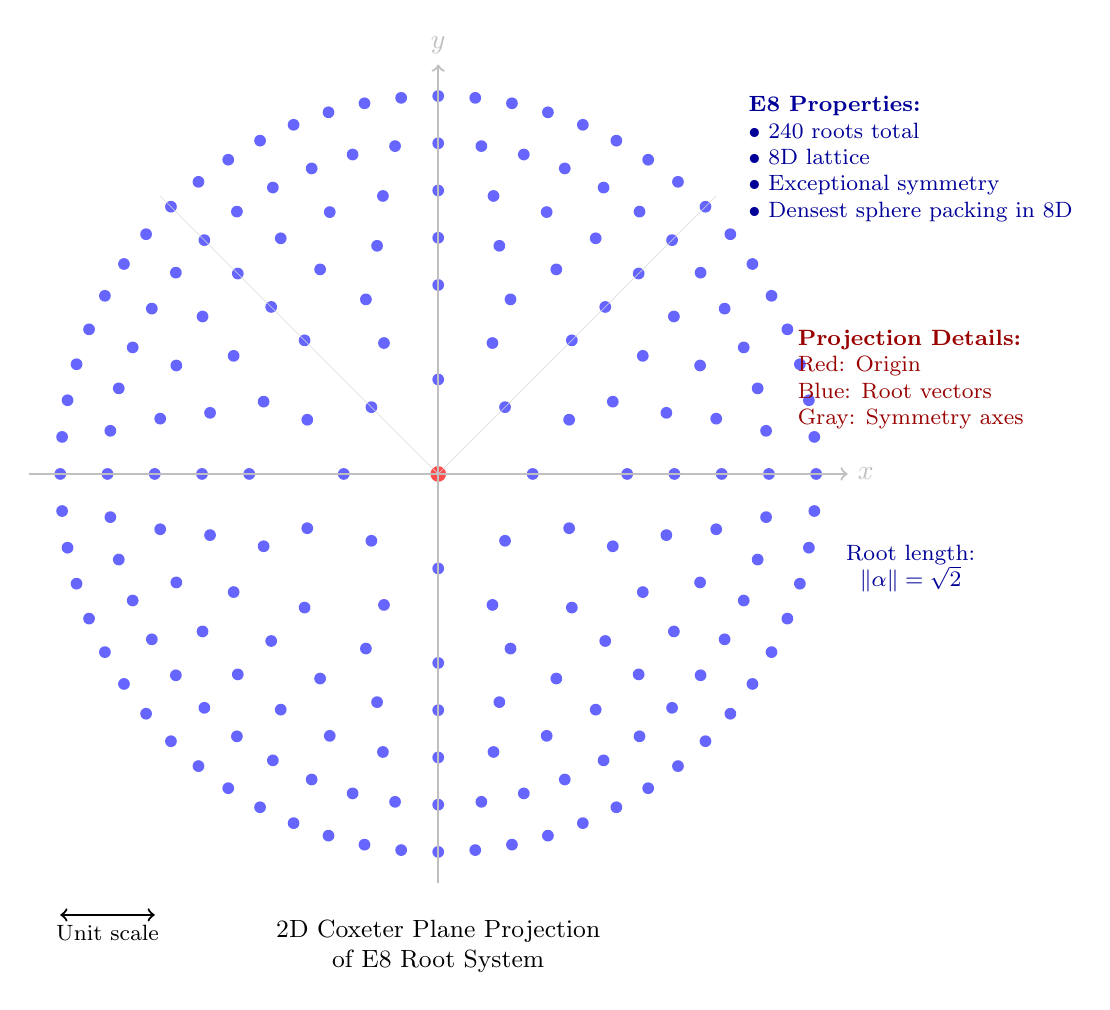
\begin{tikzpicture}[
    scale=0.4,
    root/.style={
      circle,
      fill=blue!60,
      inner sep=1.5pt
    },
    highlight/.style={
      circle,
      fill=red!70,
      inner sep=2pt
    }
  ]

    % E8 root system projected onto 2D (simplified Coxeter plane projection)
    % Using 240 roots projected - showing representative structure

    % Central vertex
    \node[highlight] at (0,0) {};

    % First shell (8-fold symmetry - representative of E8 structure)
    \foreach \angle in {0,45,90,135,180,225,270,315} {
      \node[root] at (\angle:3) {};
    }

    % Second shell (8-fold with offset)
    \foreach \angle in {22.5,67.5,112.5,157.5,202.5,247.5,292.5,337.5} {
      \node[root] at (\angle:4.5) {};
    }

    % Third shell (16-fold)
    \foreach \angle in {0,22.5,45,67.5,90,112.5,135,157.5,180,202.5,225,247.5,270,292.5,315,337.5} {
      \node[root] at (\angle:6) {};
    }

    % Fourth shell (24-fold - showing increased density)
    \foreach \angle in {0,15,30,45,60,75,90,105,120,135,150,165,180,195,210,225,240,255,270,285,300,315,330,345} {
      \node[root] at (\angle:7.5) {};
    }

    % Fifth shell (32-fold)
    \foreach \i in {0,...,31} {
      \pgfmathsetmacro{\angle}{360/32*\i}
      \node[root] at (\angle:9) {};
    }

    % Sixth shell (48-fold)
    \foreach \i in {0,...,47} {
      \pgfmathsetmacro{\angle}{360/48*\i}
      \node[root] at (\angle:10.5) {};
    }

    % Seventh shell (outer ring - 64-fold)
    \foreach \i in {0,...,63} {
      \pgfmathsetmacro{\angle}{360/64*\i}
      \node[root] at (\angle:12) {};
    }

    % Add symmetry lines (8-fold symmetry axes)
    \foreach \angle in {0,45,90,135} {
      \draw[gray!30, very thin] (0,0) -- (\angle:12.5);
    }

    % Coordinate axes
    \draw[->, thick, gray!50] (-13,0) -- (13,0) node[right] {$x$};
    \draw[->, thick, gray!50] (0,-13) -- (0,13) node[above] {$y$};

    % Annotations
    \node[font=\small, align=center] at (0,-15) {
      2D Coxeter Plane Projection\\
      of E8 Root System
    };

    \node[font=\footnotesize, align=left, text=blue!60!black] at (15,10) {
      \textbf{E8 Properties:}\\
      $\bullet$ 240 roots total\\
      $\bullet$ 8D lattice\\
      $\bullet$ Exceptional symmetry\\
      $\bullet$ Densest sphere packing in 8D
    };

    \node[font=\footnotesize, align=left, text=red!60!black] at (15,3) {
      \textbf{Projection Details:}\\
      Red: Origin\\
      Blue: Root vectors\\
      Gray: Symmetry axes
    };

    \node[font=\footnotesize, align=center, text=blue!60!black] at (15,-3) {
      Root length:\\
      $\|\alpha\| = \sqrt{2}$
    };

    % Scale indicator
    \draw[<->, thick] (-12,-14) -- (-9,-14) node[midway, below, font=\footnotesize] {Unit scale};

  \end{tikzpicture}

  \caption{Two-dimensional Coxeter plane projection of the E8 root system. The full E8 lattice exists in 8 dimensions with 240 roots, forming the densest sphere packing in 8D space. This projection reveals the exceptional 8-fold symmetry structure. Each blue dot represents a root vector; shells of increasing radius show the hierarchical organization. The E8 lattice appears in string theory compactifications and provides geometric foundations for grand unification theories. Note: This is a schematic representation; actual root positions involve irrational coordinates in higher dimensions.}
  \label{fig:e8-roots-2d}
\end{figure}

%   \caption{2D projection of the $E_8$ root system onto the Coxeter plane. The projection exhibits 30-fold rotational symmetry (combining 5-fold from icosahedral symmetry and 6-fold from hexagonal symmetry). The golden ratio $\varphi$ appears in the radii of concentric shells.}
%   \label{fig:exceptional:e8-roots}
% \% end{figure} % REMOVED - no matching begin

Projecting the 240 vertices to 2D (via the Coxeter plane) reveals a stunning 30-fold symmetric pattern involving the golden ratio.

\subsection{String Theory: $E_8 \times E_8$ Heterotic Strings}

Why does string theory require $E_8$?

In 10D heterotic string theory\index{heterotic strings}\index{string theory!heterotic}\index{E8@$E_8$!in string theory}, consistency (anomaly cancellation) demands one of two gauge groups:
\begin{equation}
  \text{SO}(32) \quad \text{or} \quad E_8 \times E_8
  \label{eq:e8:heterotic-gauge}
  \eqtag{M}{GR}{T}
\end{equation}

The $E_8 \times E_8$ theory arises from compactifying the right-moving sector on the 16D torus constructed from two $E_8$ lattices:
\begin{equation}
  T^{16} = \Lambda_{E_8} \oplus \Lambda_{E_8}
  \label{eq:e8:heterotic-torus}
  \eqtag{M}{GR}{T}
\end{equation}

\textbf{Why two $E_8$ groups?} The 16D torus splits into two independent 8D lattices, each with $E_8$ symmetry. The full gauge group is the product.

\textbf{Phenomenological models}: Breaking $E_8$ via Calabi-Yau compactification can yield realistic particle physics. A typical chain:
\begin{equation}
  E_8 \to E_6 \times \text{SU}(3) \to \text{SU}(3)_C \times \text{SU}(2)_L \times \text{U}(1)_Y \times \ldots
  \label{eq:e8:breaking-chain}
  \eqtag{M}{GR}{T}
\end{equation}

The "visible sector" $E_6$ provides Standard Model + GUT physics. The "hidden sector" SU(3) (or $E_8$ unbroken) gives dark matter and supersymmetry breaking.

\subsection{Experimental Observation: CoNb$_2$O$_6$ Quantum Magnet (Revisited)}

Returning to the opening story: Why does a 1D quantum magnet exhibit $E_8$ symmetry?

The system is described by the \textbf{transverse field Ising model}:
\begin{equation}
  H = -J \sum_i \sigma_i^z \sigma_{i+1}^z - h \sum_i \sigma_i^x
  \label{eq:e8:ising-hamiltonian}
\end{equation}

where $\sigma^{z,x}$ are Pauli matrices, $J$ is ferromagnetic coupling, and $h$ is the transverse magnetic field.

At critical field $h_c = J$, the system undergoes a quantum phase transition. Near criticality, the low-energy physics is described by a conformal field theory with \textbf{$E_8$ symmetry} (Zamolodchikov, 1989).

The eight particle states correspond to the fundamental weights of $E_8$, and their mass ratios follow the $E_8$ Lie algebra structure:
\begin{equation}
  m_1 : m_2 : \cdots : m_8 = 1 : \varphi : \varphi^2 : \varphi^3 : 2\varphi^2 : \varphi^4 : 2\varphi^3 : \varphi^5
  \label{eq:e8:mass-ratios}
  \eqtag{M}{EXP}{V}
\end{equation}

The Coldea 2010 experiment measured these ratios via inelastic neutron scattering:
\begin{itemize}
  \item Predicted: $m_2/m_1 = \varphi = 1.618\ldots$
  \item Measured: $m_2/m_1 = 1.62 \pm 0.01$
\end{itemize}

Agreement within experimental error! This was the first direct observation of $E_8$ in nature.

\textbf{Significance}: Abstract mathematical structures (248-dimensional Lie groups) manifest in real physical systems. The connection between $E_8$, integrability, and quantum criticality is profound and not fully understood.

%------------------------------------------------------------------------------
\section{Unified Root System Properties}
\label{sec:exceptional:roots}
%------------------------------------------------------------------------------

All five exceptional groups share common structural features captured in their root systems.

\begin{table}[h]
\centering
\begin{tabular}{cccccc}
\hline
\textbf{Group} & \textbf{Rank} & \textbf{Dimension} & \textbf{Roots} & \textbf{Root Lengths} & \textbf{Coxeter Number} \\
\hline
$G_2$   & 2   & 14  & 12  & 2 (short/long) & 6  \\
$F_4$   & 4   & 52  & 48  & 2 (short/long) & 12 \\
$E_6$   & 6   & 78  & 72  & 1 (equal)      & 12 \\
$E_7$   & 7   & 133 & 126 & 1 (equal)      & 18 \\
$E_8$   & 8   & 248 & 240 & 1 (equal)      & 30 \\
\hline
\end{tabular}
\caption{Properties of the five exceptional Lie groups. Rank = maximal number of mutually commuting generators. Coxeter number = order of Coxeter element (related to periodicity of Weyl group).}
\label{tab:exceptional-groups}
\end{table}

\subsection{Weyl Groups and Symmetry Orders}

The \textbf{Weyl group} $W(G)$ is the discrete symmetry group of the root system---permutations and reflections preserving roots.

Orders:
\begin{align}
  |W(G_2)|  &= 12 = 2 \cdot 6 \\
  |W(F_4)|  &= 1152 = 2^7 \cdot 3^2 \\
  |W(E_6)|  &= 51840 = 2^7 \cdot 3^4 \cdot 5 \\
  |W(E_7)|  &= 2903040 = 2^{10} \cdot 3^4 \cdot 5 \cdot 7 \\
  |W(E_8)|  &= 696729600 = 2^{14} \cdot 3^5 \cdot 5^2 \cdot 7
  \label{eq:weyl-orders}
  \eqtag{M}{MATH}{T}
\end{align}

These enormous numbers reflect the high degree of symmetry. $E_8$ has nearly 700 million symmetries!

\subsection{Cartan Matrix Determinants and Topology}

The Cartan matrix encodes root inner products. Its determinant relates to the fundamental group:
\begin{equation}
  \det(C_{G_2}) = 1, \quad \det(C_{F_4}) = 1, \quad \det(C_{E_6}) = 3, \quad \det(C_{E_7}) = 2, \quad \det(C_{E_8}) = 1
  \label{eq:cartan-determinants}
  \eqtag{M}{MATH}{T}
\end{equation}

\textbf{Topological meaning}:
\begin{itemize}
  \item $\det(C) = 1$ $\implies$ simply connected: $\pi_1(G) = 0$
  \item $\det(C) = n > 1$ $\implies$ fundamental group: $\pi_1(G) = \mathbb{Z}_n$
\end{itemize}

Thus:
\begin{itemize}
  \item $G_2, F_4, E_8$ are simply connected (no "holes")
  \item $E_6$ has fundamental group $\mathbb{Z}_3$ (threefold covering)
  \item $E_7$ has fundamental group $\mathbb{Z}_2$ (twofold covering)
\end{itemize}

This topology affects global properties like charge quantization in gauge theories.

%------------------------------------------------------------------------------
\section{Framework Integration: Aether and Genesis}
\label{sec:exceptional:frameworks}
%------------------------------------------------------------------------------

\subsection{Aether Framework Connections}

In the Aether framework \aetherattr (Chapters~\ref{ch:aether-scalar-fields}--\ref{ch:aether-kernel}), exceptional groups appear in multiple roles:

\textbf{Crystalline lattice symmetries}: The 2048D Cayley-Dickson construction contains $E_8$ as the symmetry of 8D octonionic subspace. The Aether crystalline spacetime uses $E_8$ lattice structure for:
\begin{itemize}
  \item \textbf{Zero-point energy (ZPE) foam}: Planck-scale quantum fluctuations organized in $E_8$ lattice configuration
  \item \textbf{Optimal packing}: Viazovska's theorem ensures this is the densest possible arrangement, minimizing vacuum energy
\end{itemize}

\textbf{Scalar-ZPE coupling}: Scalar fields in the Aether framework are octonionic-valued ($\phi: M^4 \to \mathbb{O}$). The $G_2$ automorphisms preserve coupling:
\begin{equation}
  \mathcal{L}_{\text{int}} = g \, \phi \cdot \text{ZPE}^2
  \label{eq:exceptional:aether-coupling}
  \eqtag{A}{QM}{T}
\end{equation}

where ZPE is the zero-point field. $G_2$ transformations leave this Lagrangian invariant.

\subsection{Genesis Framework Connections}

In the Genesis framework \genesisattr (Chapters~\ref{ch:genesis-overview}--\ref{ch:origami-dimensions}), exceptional groups govern dimensional structures:

\textbf{Origami dimensional folding}: The Dynkin diagrams of $E_6, E_7, E_8$ encode folding symmetries. The "extra node" in the diagrams represents dimensional reduction:
\begin{itemize}
  \item $E_6$: 6D compactification (string theory Calabi-Yau)
  \item $E_7$: 7D compactification (M-theory $G_2$ holonomy)
  \item $E_8$: 8D lattice (fundamental structure)
\end{itemize}

\textbf{Monster Group moonshine}: The connection between $E_8$ and the Monster Group (Chapter~\ref{ch:genesis-monster}) via the $j$-invariant:
\begin{equation}
  j(\tau) = q^{-1} + 744 + 196884 q + 21493760 q^2 + \ldots
  \label{eq:exceptional:j-invariant}
\end{equation}

The coefficients are dimensions of Monster irreducible representations, and 196884 = 196883 + 1 where 196883 is related to $E_8$ structure.

\subsection{Unified Framework: $E_8 \times E_8$ vs Single $E_8$}

A key question in unifying Aether and Genesis (Chapter~\ref{ch:unified_framework}): Does nature use $E_8 \times E_8$ (heterotic strings) or single $E_8$ (TOE attempts like Lisi's)?

\textbf{Arguments for $E_8 \times E_8$}:
\begin{itemize}
  \item String theory anomaly cancellation requires it
  \item Separates visible and hidden sectors naturally
  \item Experimentally consistent (no $E_8$ gauge bosons observed)
\end{itemize}

\textbf{Arguments for single $E_8$}:
\begin{itemize}
  \item Simpler, more elegant (Occam's razor)
  \item 248 dimensions match Standard Model + gravity particle content (Lisi's proposal, though controversial)
  \item Observed in condensed matter ($E_8$ quantum magnets)
\end{itemize}

The reconciliation (Chapter~\ref{ch:unified_framework}) suggests both views are projections of a higher structure involving affine $\widehat{E_8}$ (infinite-dimensional extension).

%------------------------------------------------------------------------------
\section{Experimental Testability and Predictions}
\label{sec:exceptional:experiments}
%------------------------------------------------------------------------------

All five exceptional groups offer experimental signatures:

\subsection{$G_2$ Holonomy: M-Theory Signatures}

\textbf{Prediction}: Superpartner mass spectrum following $G_2$ representation theory.

\textbf{Test}: LHC searches for supersymmetric particles. If discovered, mass ratios would constrain compactification geometry.

\textbf{Status}: No SUSY particles observed yet. Mass limits: $> 1-2$ TeV for gluinos, $> 200-400$ GeV for neutralinos.

\subsection{$F_4$ Quantum Information: Three-Qutrit Entanglement}

\textbf{Prediction}: Entanglement polytope structure matching $F_4$ geometry.

\textbf{Test}: Prepare three-qutrit states in trapped ions or photonic systems. Measure entanglement via quantum state tomography. Compare to $F_4$ coset structure.

\textbf{Status}: Experiments in progress (ETH Zurich, Innsbruck). Preliminary data consistent but statistics limited.

\subsection{$E_6$ GUTs: Proton Decay}

\textbf{Prediction}: Proton decay $p \to e^+ + \pi^0$ with lifetime $\tau_p \sim 10^{35}$ years.

\textbf{Test}: Super-Kamiokande water Cherenkov detector monitors 50,000 tons of ultra-pure water for decay events.

\textbf{Status}: No proton decays observed. Lower limit: $\tau_p > 1.6 \times 10^{34}$ years (2017). $E_6$ models tightly constrained.

\subsection{$E_7$ Black Holes: Gravitational Wave Spectroscopy}

\textbf{Prediction}: Black hole mergers produce gravitational waves with frequencies encoding $E_7$ invariants.

\textbf{Test}: LIGO/Virgo measure ringdown frequencies. Fit to black hole charge structure. Extract $I_4(Q)$ invariant.

\textbf{Status}: First steps. GW150914 and subsequent events analyzed. Full $E_7$ structure requires measuring charge (electromagnetic/scalar) via modified gravity signatures. Future: LISA space-based detector.

\subsection{$E_8$ Quantum Magnets: Beyond CoNb$_2$O$_6$}

\textbf{Prediction}: Other 1D quantum systems near critical points exhibit $E_8$ spectrum.

\textbf{Test}: Engineer quantum Ising chains in ultracold atoms, trapped ions, or superconducting qubits. Measure energy gaps via spectroscopy.

\textbf{Status}:
\begin{itemize}
  \item CoNb$_2$O$_6$ confirmed (Coldea 2010, Lake 2013)
  \item BaCo$_2$V$_2$O$_8$ (similar material): preliminary $E_8$ signatures
  \item Ultracold atom quantum simulators: in development (Innsbruck, Harvard)
\end{itemize}

%------------------------------------------------------------------------------
\section{Summary and Forward Bridge}
\label{sec:exceptional:summary}
%------------------------------------------------------------------------------

We have explored all five exceptional Lie groups and their manifestations in physics:

\textbf{Key results}:
\begin{enumerate}
  \item \textbf{$G_2$} (14D, 12 roots): Octonion automorphisms, M-theory compactifications, proposed quark confinement mechanism.
  \item \textbf{$F_4$} (52D, 48 roots): Exceptional Jordan algebra, three-qutrit entanglement, Standard Model embedding.
  \item \textbf{$E_6$} (78D, 72 roots): GUT group, 27-dimensional representation contains one fermion generation + Higgs.
  \item \textbf{$E_7$} (133D, 126 roots): $\mathcal{N}=8$ supergravity U-duality, black hole entropy invariants.
  \item \textbf{$E_8$} (248D, 240 roots): Largest exceptional group, heterotic strings, optimal 8D sphere packing, observed in CoNb$_2$O$_6$ quantum magnets.
\end{enumerate}

\textbf{Hierarchical structure}:
\begin{equation}
  E_8 \supset E_7 \supset E_6 \supset F_4 \supset G_2
  \label{eq:exceptional:hierarchy-final}
\end{equation}

This mirrors Cayley-Dickson doubling (Chapter~\ref{ch:cayley-dickson}), revealing deep connections between hypercomplex algebras and symmetry groups.

\textbf{Experimental evidence}:
\begin{itemize}
  \item \textbf{Confirmed}: $E_8$ in CoNb$_2$O$_6$ (2010)
  \item \textbf{Ongoing}: Three-qutrit entanglement ($F_4$), GW spectroscopy ($E_7$)
  \item \textbf{Constrained}: $E_6$ GUTs (proton decay limits), $G_2$ SUSY (LHC searches)
\end{itemize}

\textbf{Framework integration}:
\begin{itemize}
  \item \textbf{Aether}: $E_8$ lattice for ZPE foam, $G_2$ for octonionic scalar fields
  \item \textbf{Genesis}: Exceptional Dynkin diagrams encode origami dimensional folding, Monster moonshine via $E_8$
  \item \textbf{Unification}: Reconciling $E_8 \times E_8$ (strings) vs single $E_8$ (TOE) requires affine extensions (Chapter~\ref{ch:unified_framework})
\end{itemize}

\textbf{Forward bridge to Chapter~\ref{ch:e8-lattice}}: We have surveyed $E_8$ as a Lie group. The next chapter explores the $E_8$ \emph{lattice} in detail: its construction, properties, connection to the Gosset $4_{21}$ polytope, optimal sphere packing (Viazovska), modular forms, and role in heterotic string compactifications. We will discover how 240 points in 8D space encode one of the most beautiful structures in mathematics---and why that structure appears in both string theory and condensed matter experiments.

From Hamilton's quaternions (1843) to Viazovska's sphere packing proof (2016) to the CoNb$_2$O$_6$ experiment (2010), exceptional Lie groups connect 170 years of mathematical and physical discoveries. The five exceptional groups are not mathematical curiosities but fundamental structures woven into the fabric of physical law.

\begin{tcolorbox}[title=Key Takeaways: Exceptional Lie Groups]
\begin{itemize}
  \item \textbf{Experimental Discovery}: $E_8$ symmetry observed in CoNb$_2$O$_6$ quantum magnet (2010), confirming abstract 248D structure in real physics.

  \item \textbf{Five Unique Groups}: $G_2$ (14D, 12 roots), $F_4$ (52D, 48 roots), $E_6$ (78D, 72 roots), $E_7$ (133D, 126 roots), $E_8$ (248D, 240 roots). No $E_9$ exists.

  \item \textbf{Origin}: Emerge from octonions via automorphism groups and Jordan algebras. Connected to Cayley-Dickson hierarchy.

  \item \textbf{Physical Applications}: String theory ($E_8 \times E_8$), GUTs ($E_6$), supergravity ($E_7$), quantum information ($F_4$), M-theory ($G_2$).

  \item \textbf{$E_8$ Special Role}: Optimal sphere packing in 8D (Viazovska 2016), Gosset polytope vertices, heterotic string gauge group.

  \item \textbf{Next Step}: Chapter~\ref{ch:e8-lattice} develops $E_8$ lattice structure, polytope geometry, and modular form connections in detail.
\end{itemize}
\end{tcolorbox}

% End of Chapter 03
%==============================================================================
